% Source of the figure threading.pdf (the threading operation: a chain link before and after a thread is threaded through it).
% Compile with pdfLaTeX; the PDF is included in the manuscript at its natural size.
\documentclass[tikz,border=1pt]{standalone}
\usepackage[T1]{fontenc}
\usepackage{stix}
\pdfinfoomitdate=1 \pdftrailerid{} \pdfsuppressptexinfo=-1
\definecolor{threadred}{RGB}{200,40,40}
\begin{document}
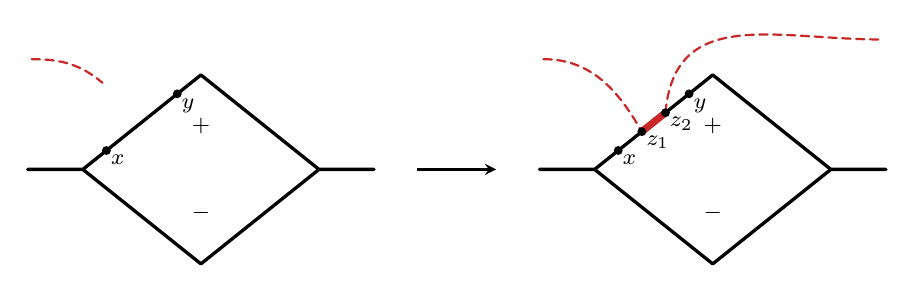
\begin{tikzpicture}[x=1cm, y=1cm,
    chain/.style={line width=1.2pt, line cap=round, line join=round},
    thread/.style={line width=0.8pt, line cap=round},
    crossing/.style={line width=2.6pt, line cap=butt},
    lead/.style={thread, densely dashed}]
  % A chain link with the two single edges next to it: #1 = x-coordinate of its center.
  % The upper path is the positive path, the lower path the negative path.
  \newcommand{\chainlink}[1]{%
    \draw[chain] (#1-2.2,0) -- (#1-1.5,0) -- (#1,1.2) -- (#1+1.5,0) -- (#1+2.2,0);
    \draw[chain] (#1-1.5,0) -- (#1,-1.2) -- (#1+1.5,0);
    \node at (#1,0.55) {\footnotesize $+$};
    \node at (#1,-0.55) {\footnotesize $-$};}
  % A vertex on the positive path with its name inside the link: #1 = coordinate, #2 = name.
  \newcommand{\pathvertex}[2]{%
    \fill (#1) circle[radius=1.6pt];
    \node[anchor=north west, inner sep=1.5pt] at (#1) {\footnotesize #2};}

  \useasboundingbox (0.15,-1.3) rectangle (11.05,1.8);
  % before: the thread ends in front of the selected edge {x,y} of the positive path
  \chainlink{2.35}
  \draw[lead, threadred] (0.2,1.4) to[out=0, in=140] (1.1,1.1);
  \pathvertex{1.15,0.24}{$x$}
  \pathvertex{2.05,0.96}{$y$}

  \draw[line width=0.8pt, -stealth] (5.1,0) -- (6.1,0);

  % after: the edge is subdivided into x-z_1-z_2-y and the thread runs through the crossing edge {z_1,z_2}
  \chainlink{8.85}
  \draw[lead, threadred] (6.7,1.4) to[out=0, in=120] (7.95,0.48);
  \draw[lead, threadred] (8.25,0.72) to[out=85, in=180, looseness=1.2] (11.0,1.65);
  \draw[crossing, threadred] (7.95,0.48) -- (8.25,0.72);
  \pathvertex{7.65,0.24}{$x$}
  \pathvertex{7.95,0.48}{$z_1$}
  \pathvertex{8.25,0.72}{$z_2$}
  \pathvertex{8.55,0.96}{$y$}
\end{tikzpicture}
\end{document}
